\section{Durchführung}
\label{sec:Durchführung}
\subsection{Versuchaufbau}
Der Versuchsaufbau ist in Abbildung (\ref{ig:Foto}) zu sehen. Dieser besteht aus einem Michelson Interferometer in welches eine Gaszelle eingebaut ist, sodass 
der Lichtstrahl durch die Gaszelle fällt, der vom verschiebbaren Spiegel reflektiert wird. Außerdem fällt das Interferenzmuster auf eine Photodiode, die die 
Minima und Maxima Wechsel misst. Die Messung aus der Photodiode wird mithilfe eines Schmitt-Triggers in einen Puls umgewandelt. Die Anzahl der Pulse werden 
auf einem Bildschirm angezeigt. 
\begin{figure}[H]
    \centering
    %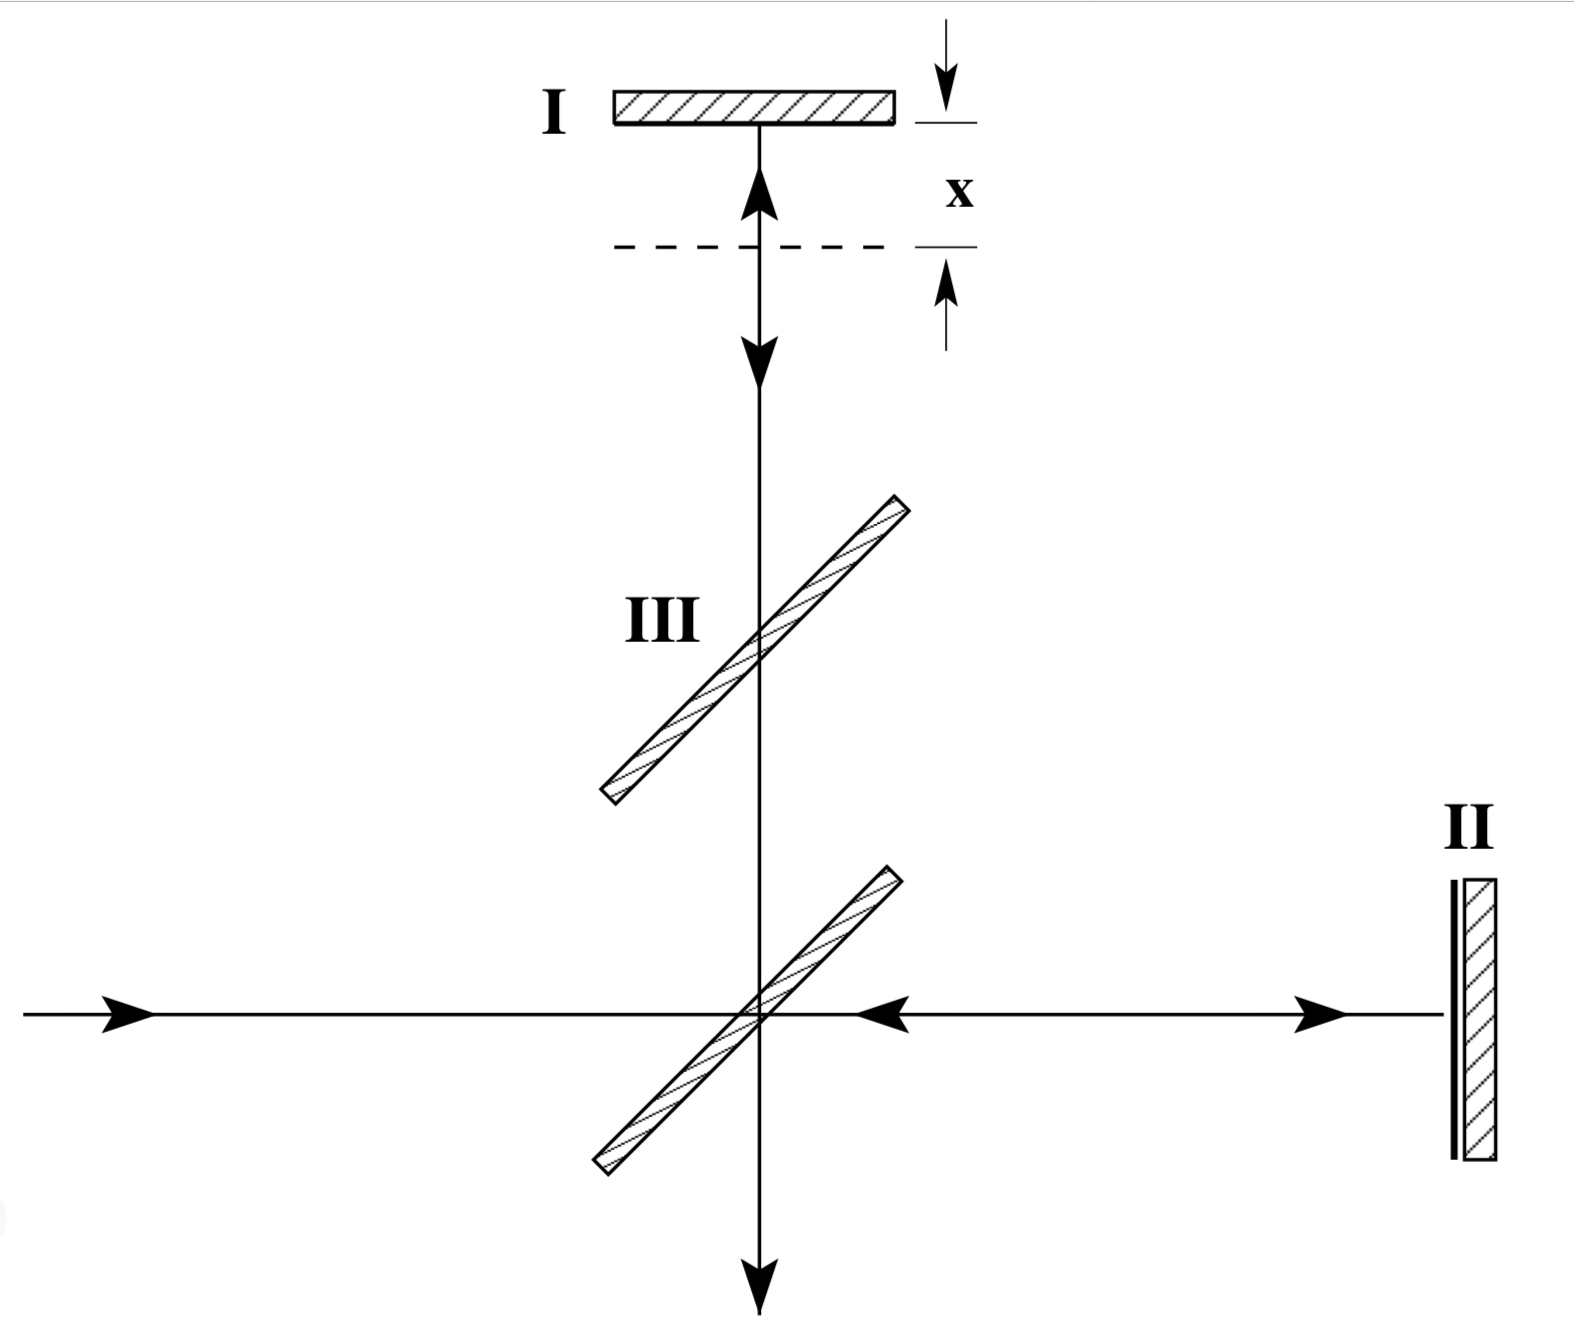
\includegraphics[width=0.6\linewidth]{"content/Bilder/V401.png"}
    \caption{Foto des Versuchsaufbau mit Strahlengang \cite{anleitungV401}.}
    \label{fig:Foto}
\end{figure}
\subsection{Versuchsdurchführung}
Zu Begin des Versuchs wird der Spiegel, dessen Abstand sich im Verlauf des Versuchs nicht ändert, justiert, sodass ein Interferenzmuster auf der 
Photodiode entsteht. Im Anschluss wird der bewegbare Spiegel mithilfe einer motorisierten Mikrometerschraube im Bereich von $6$ bis $11 \, \unit{\centi\meter}$ 
kontinuierlich verschoben. Währenddessen werden von der Photodiode die Minimums und Maximumswechsel gemessen und die Gesamtanzahl dargestellt. Diese Messung 
wird insgesamt 10 Mal gemacht. \\
Danach wird die Gaszelle evakuiert und die Pulszahl während der Evakuierung und beim Lufthereinlassen notiert. Beide Anzahlen werden jeweils 5 Mal gemessen. 
